\documentclass[aagreenthesis]{subfiles}
%\usepackage{macros}
\begin{document}
\chapter{chirality on demand: the discovery of activated Chirality in ahiral
bent-core mesogens}
\section{A history of de Vries phases in liquid crystals}
\section{Characteristic behaviour of the bent-core de Vries phase}
\subsection{Textures of bent-code de Vries phase}

\begin{figure}[h!]
    \centering
    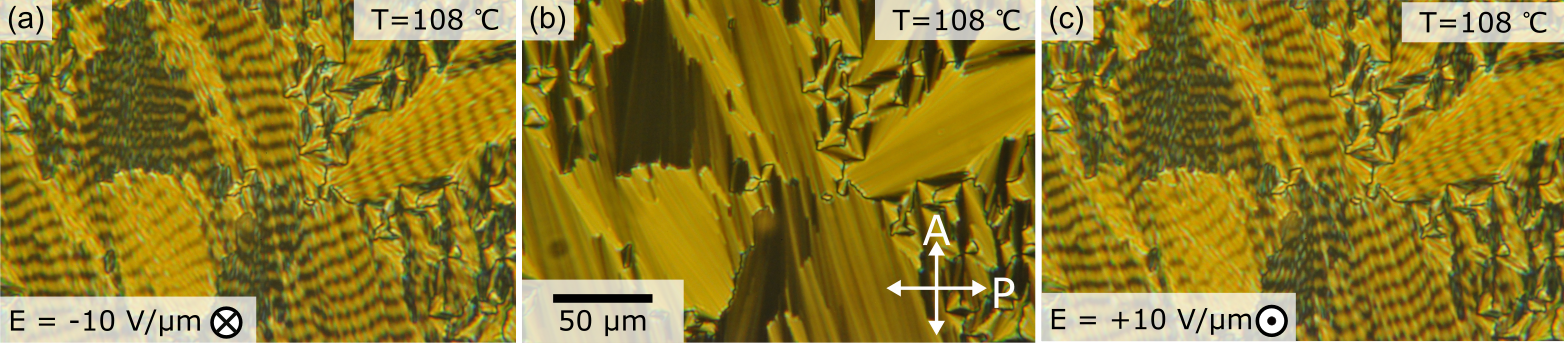
\includegraphics[width=.8\textwidth]{figs/pal30/textureSM2/sm1Textures100.png}
    \caption{\label{}}
\end{figure}


\subsection{Electro-optics of bent-core de Vries phase}
text
\begin{figure}[h!]
    \centering
    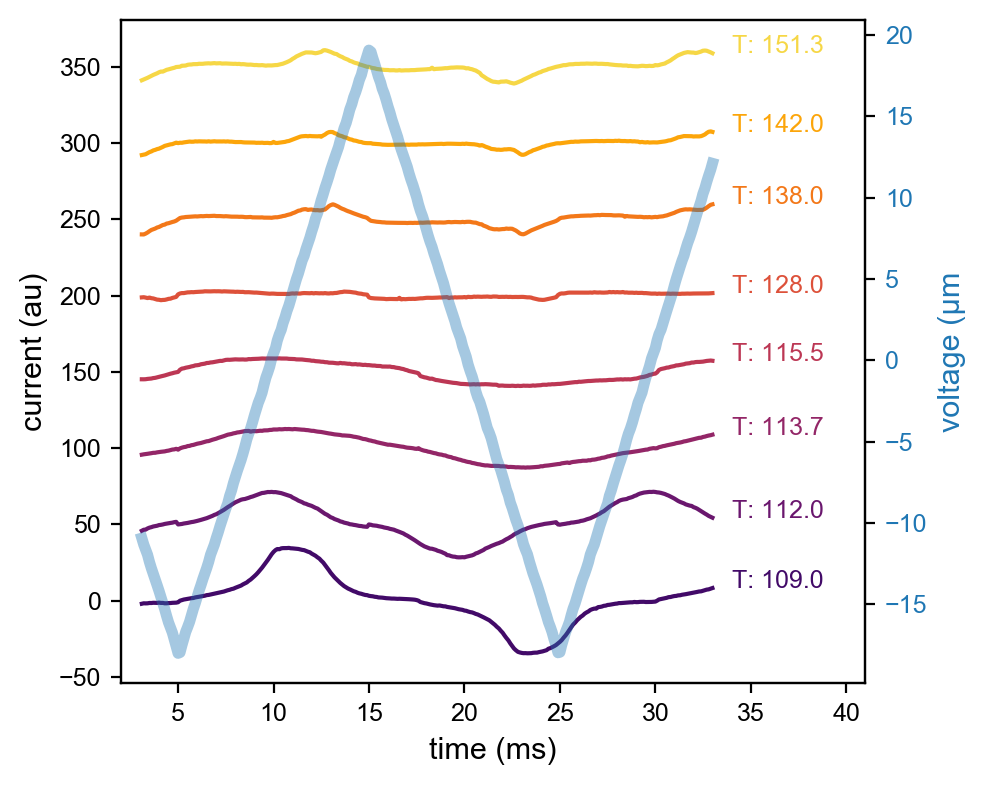
\includegraphics[width=.8\textwidth]{figs/pal30/prc/spacedSm1PRC.png}
    \caption{\label{}}
\end{figure}
text

\begin{figure}[h!]
    \centering
    \includegraphics[width=.8\textwidth]{figs/pal30/prc/3dplot-sm1.png}
    \caption{\label{}}
\end{figure}
text

\subsection{X-ray analysis of bent-core de Vries phase}

\begin{figure}[h!]
    \centering
    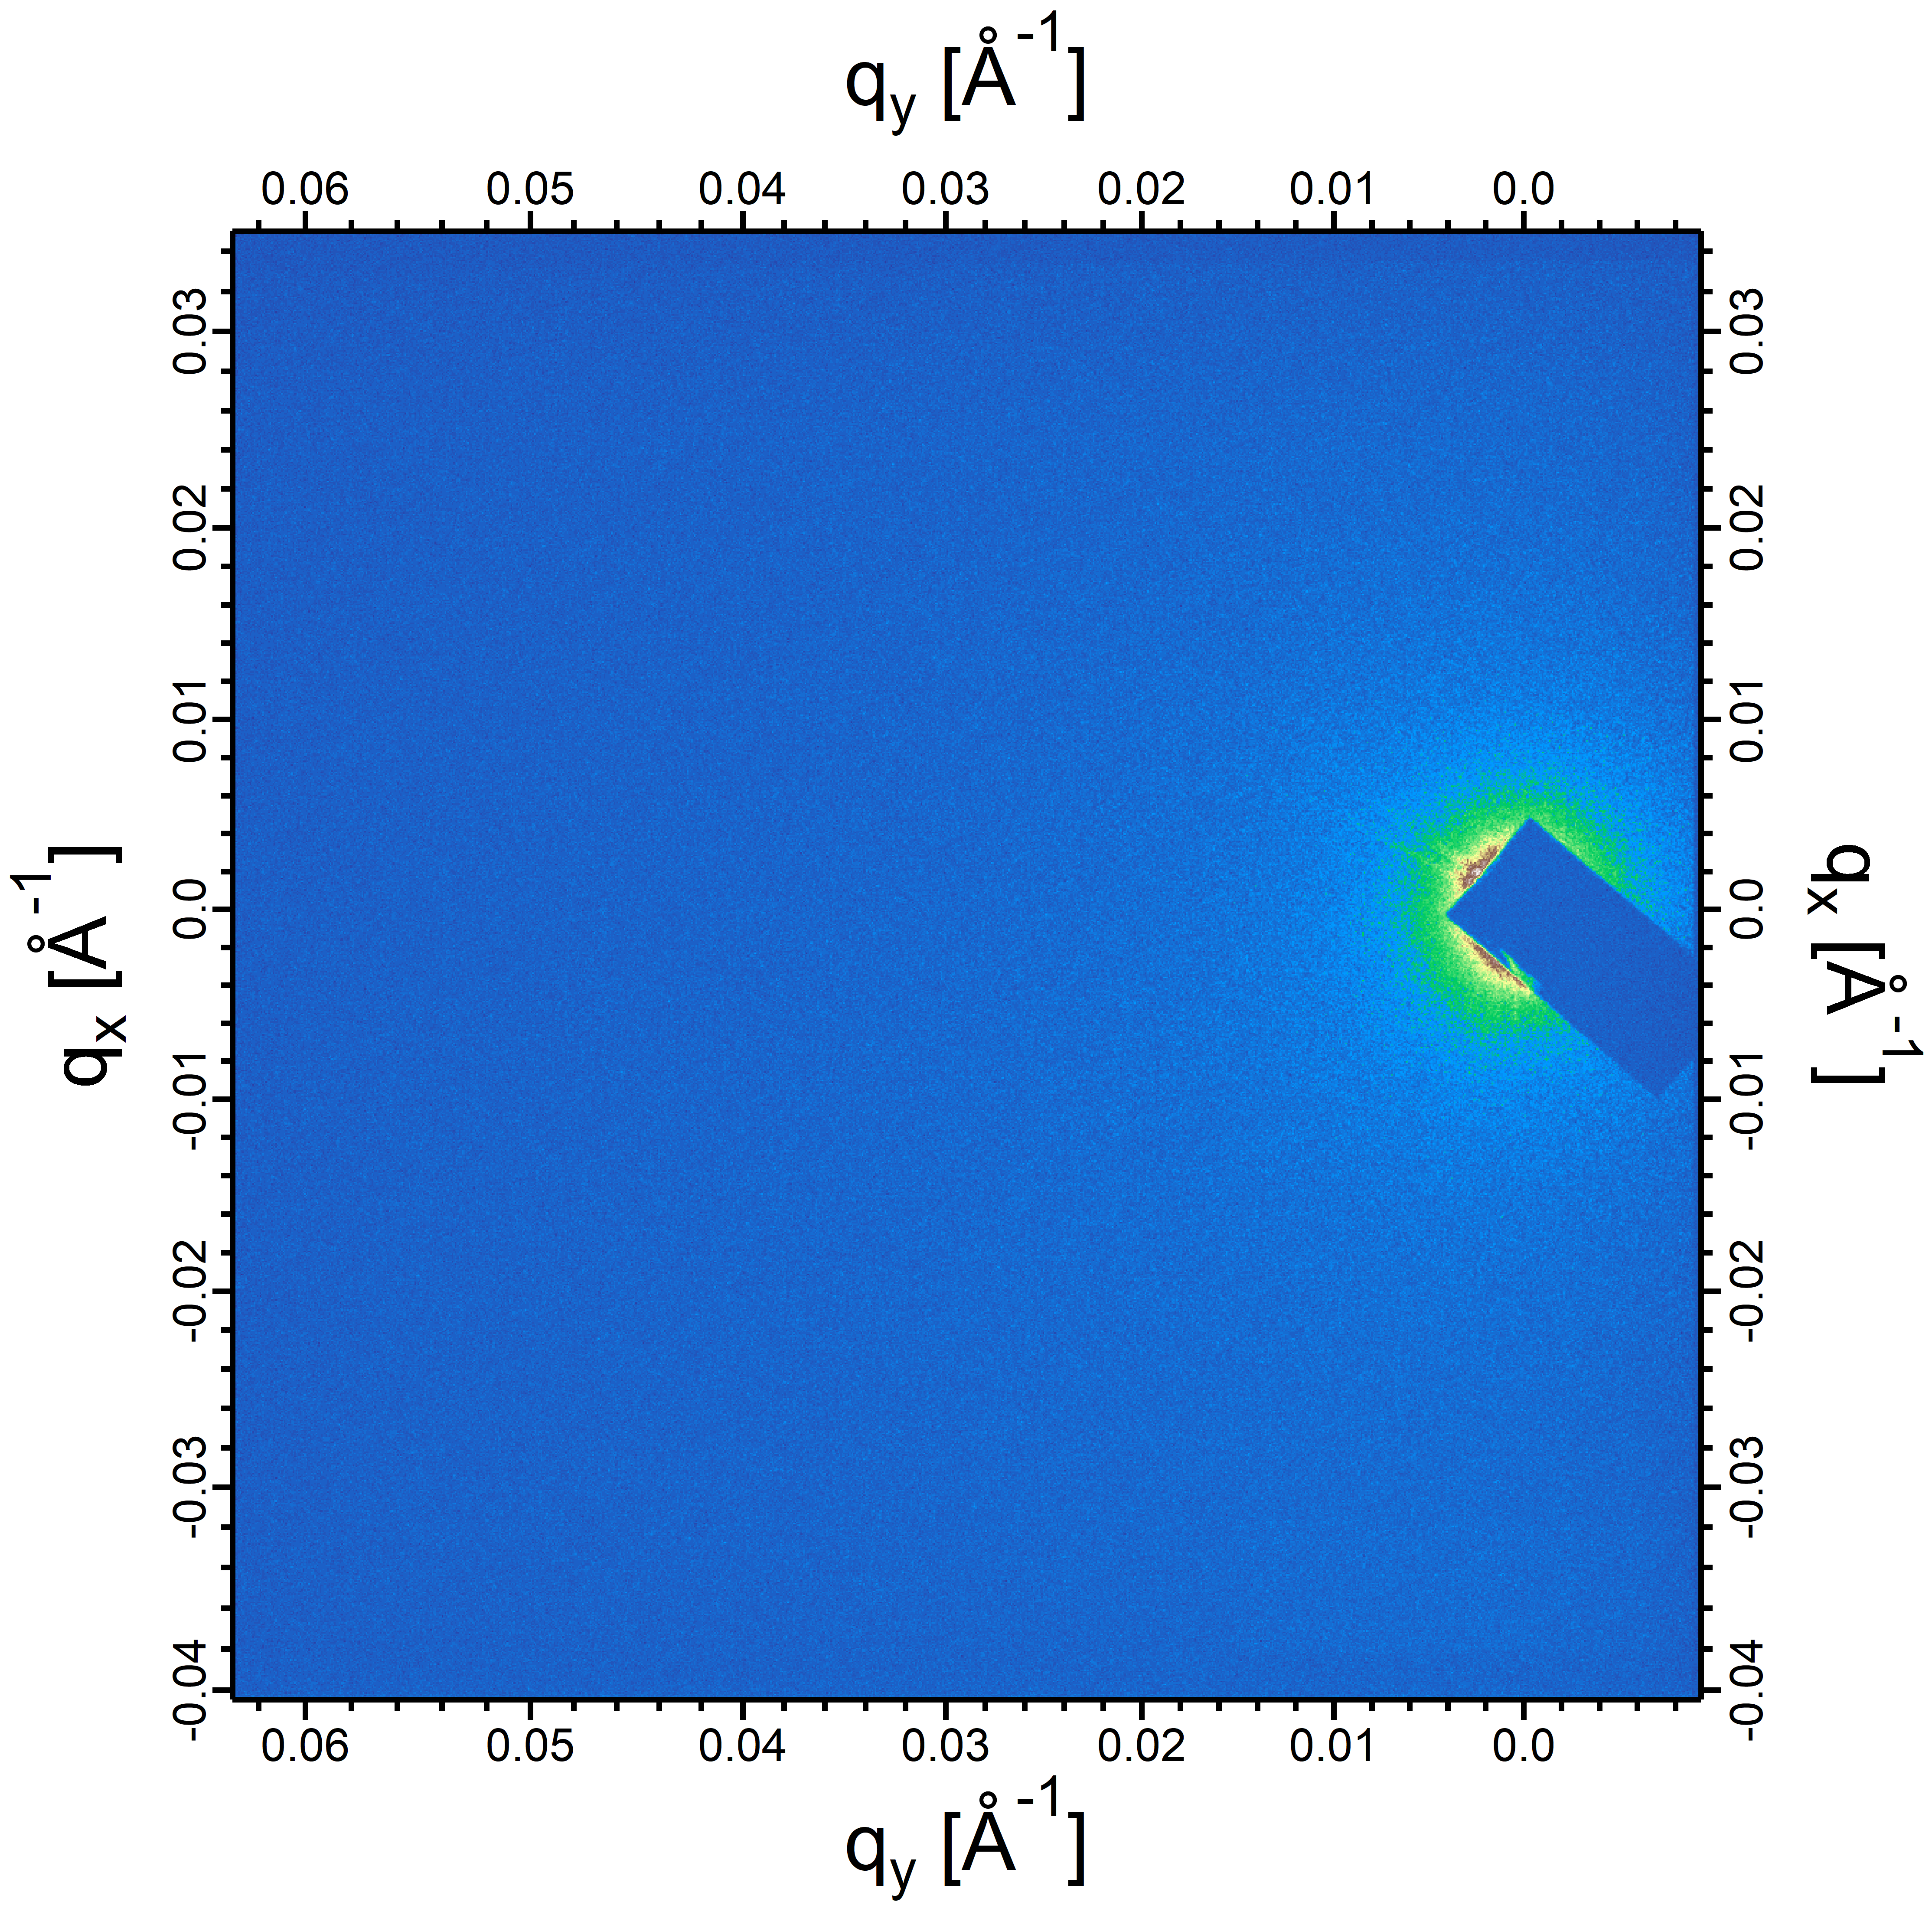
\includegraphics[width=.8\textwidth]{figs/pal30/xraysm1/rsosxSmaT113-modified.png}
    \caption{\label{}}
\end{figure}


\begin{figure}[h!]
    \centering
    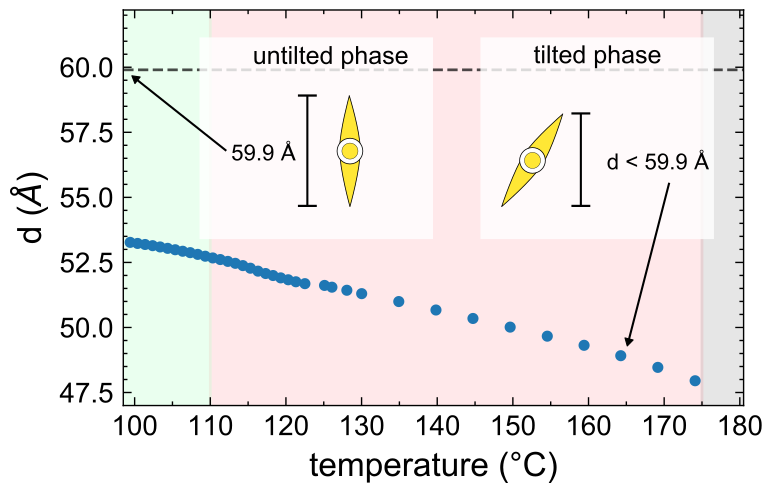
\includegraphics{figs/pal30/xraysm1/sm1-saxs-annote.png}
    \caption{\label{}}
\end{figure}




\section{Discussion for the bent-core de Vries phase}
\begin{figure}[h!]
    \centering
    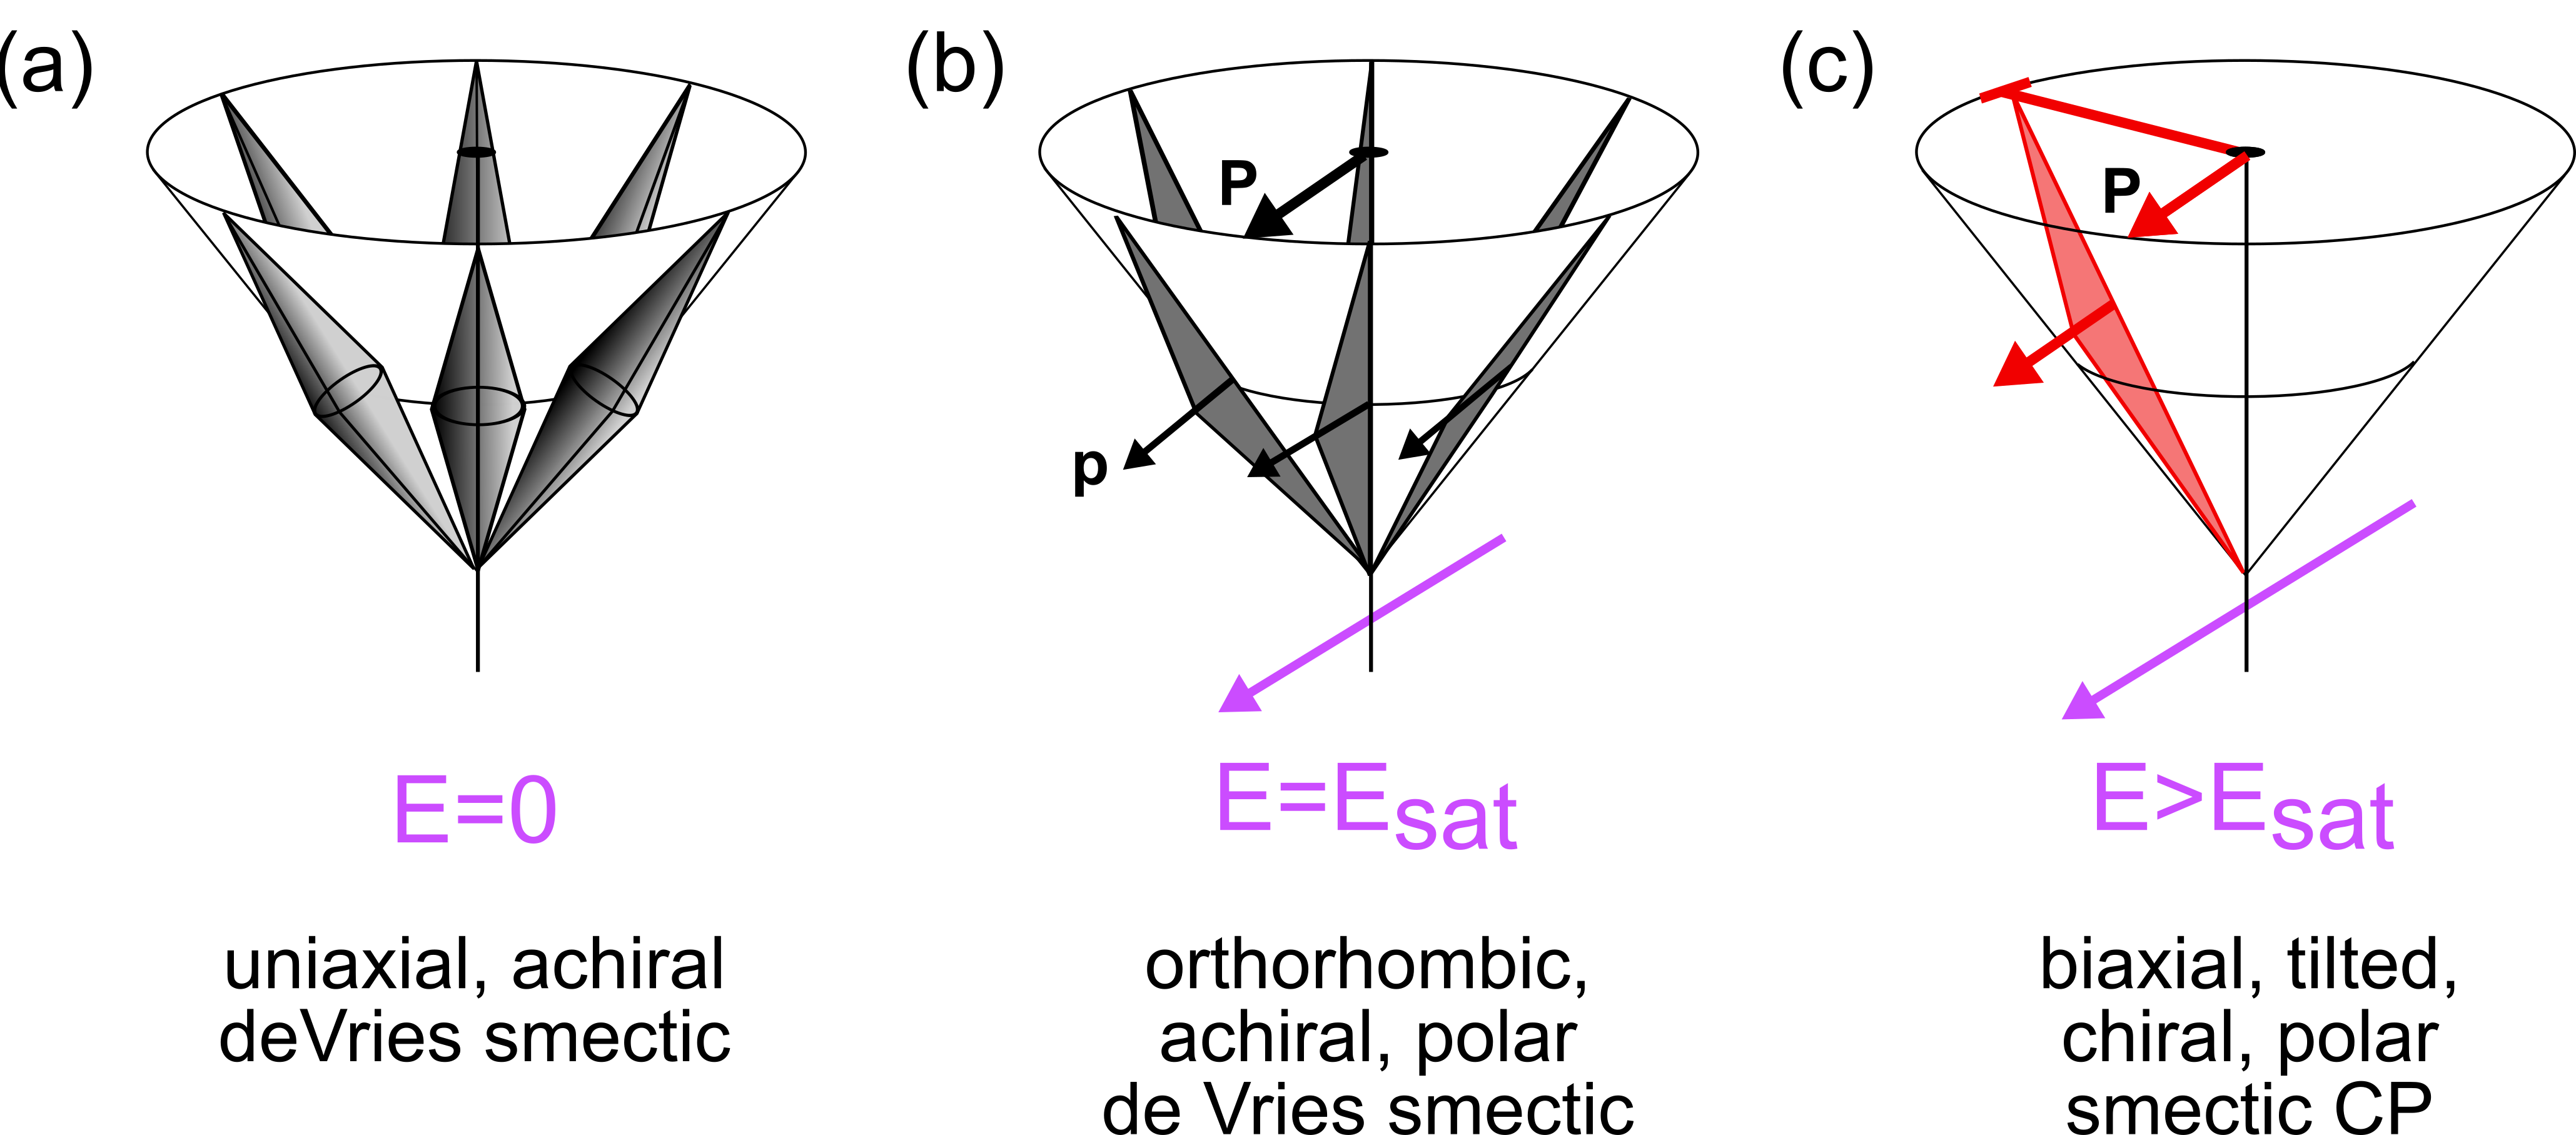
\includegraphics{figs/pal30/deVries/dvAlign.png}
    \caption{\label{}}
\end{figure}




\biblio
\end{document}


